% !TEX TS-program = pdflatex
% !TEX encoding = UTF-8 Unicode

% This is a simple template for a LaTeX document using the "article" class.
% See "book", "report", "letter" for other types of document.

\documentclass[11pt]{article} % use larger type; default would be 10pt

\usepackage[utf8]{inputenc} % set input encoding (not needed with XeLaTeX)

%%% Examples of Article customizations
% These packages are optional, depending whether you want the features they provide.
% See the LaTeX Companion or other references for full information.

%%% PAGE DIMENSIONS
\usepackage{geometry} % to change the page dimensions
\geometry{letterpaper,margin=1in} % or letterpaper (US) or a5paper or....
% \geometry{margin=2in} % for example, change the margins to 2 inches all round
% \geometry{landscape} % set up the page for landscape
%   read geometry.pdf for detailed page layout information

\usepackage{graphicx} % support the \includegraphics command and options

% \usepackage[parfill]{parskip} % Activate to begin paragraphs with an empty line rather than an indent

%%% PACKAGES
\usepackage{booktabs} % for much better looking tables
\usepackage{array} % for better arrays (eg matrices) in maths
\usepackage{paralist} % very flexible & customisable lists (eg. enumerate/itemize, etc.)
\usepackage{verbatim} % adds environment for commenting out blocks of text & for better verbatim
%\usepackage{subfig} % make it possible to include more than one captioned figure/table in a single float
\usepackage{caption}
\usepackage[singlelinecheck=on,labelformat=simple]{subcaption}
	\renewcommand\thesubfigure{(\alph{subfigure})}
	\renewcommand\thesubtable{(\alph{subtable})}
\usepackage{hyperref}
  \hypersetup{colorlinks   = true, urlcolor= blue, linkcolor=black,citecolor=blue}
\usepackage{natbib}
\usepackage[section]{placeins} %keep figure in section
\usepackage{setspace} %for double space
\usepackage{amsmath}
\usepackage{amsfonts}

%%% HEADERS & FOOTERS
\usepackage{fancyhdr} % This should be set AFTER setting up the page geometry
\pagestyle{fancy} % options: empty , plain , fancy
\renewcommand{\headrulewidth}{0pt} % customise the layout...
\lhead{}\chead{}\rhead{}
\lfoot{}\cfoot{\thepage}\rfoot{}

%%% SECTION TITLE APPEARANCE
\usepackage{sectsty}
\allsectionsfont{\sffamily\mdseries\upshape} % (See the fntguide.pdf for font help)
% (This matches ConTeXt defaults)

%%% ToC (table of contents) APPEARANCE
\usepackage[nottoc,notlof,notlot]{tocbibind} % Put the bibliography in the ToC
\usepackage[titles,subfigure]{tocloft} % Alter the style of the Table of Contents
\renewcommand{\cftsecfont}{\rmfamily\mdseries\upshape}
\renewcommand{\cftsecpagefont}{\rmfamily\mdseries\upshape} % No bold!

%%% END Article customizations

%%% The "real" document content comes below...
\graphicspath{{./images/}}
\begin{document}
\begin{titlepage}
	
	\begin{center}
		\vspace{10cm}
		
		% Upper part of the page
		
\includegraphics[width=.5\textwidth]{./images/primarylogo}\\[3cm]    
		
		\normalsize EE 227C\\
		\textsc{\large Convex Optimization}\\[1cm]		
		
		% Title
		\hrule 
		\vspace{1 cm}
		{ \Large \textbf{Semidefinite Programming Relaxations of Constraint Satisfaction Problems}\\[0.5cm]
			\vspace{0.5 cm}
			\hrule
			\vspace{1.5 cm}
			
			% Author and supervisor
			\begin{minipage}[t]{0.4\textwidth}
				\begin{flushleft} \large
					\emph{Authors:}\\
					\vspace{0.7ex}
					Riley \textsc{Murray} \\
					Paul \textsc{Anderson}
					
				\end{flushleft}
			\end{minipage}
			\begin{minipage}[t]{0.4\textwidth}
				\begin{flushright} \large
					\emph{Instructor:} \\
					\vspace{0.7ex}
					Benjamin \textsc{Recht}\\[0.3 cm]
				\end{flushright}
			\end{minipage}
			\vfill 
			% Bottom of the page
			University of California, Berkeley\\[.5cm]
			\large \today}
		
	\end{center}
	
\end{titlepage}

\section*{Abstract}

Content goes here

\section{Introduction}

A Constraint Satisfaction Problem (CSP) is a discrete optimization problem consisting of a set of variables ( which take on values in a finite domain) and a set of constraints (indicator functions defined on a subset of variables of some specified cardinality).

The goal is to assign each variable a value in the domain so that the largest number of constraints are satisfied.

CSP's subsume a wide range of fundamental combinatorial optimization problems, including Max k-SAT, graph coloring (approximately defined), and Unique Games.

Significant effort has been dedicated to developing approximation algorithms for CSP's. The most general of these algorithms involve solving a canonical SDP relaxation of the CSP, (which we call ``Basic SDP" \citep{raghavendra2008optimal}) and use extremely sophisticated post-processing of SDP vectors to determine an assignment of variables. Unfortunately, as was shown in \cite{qwivedi2015introduction}, these algorithms require impossibly powerful machines.

In this work, we deploy approximation algorithms rooted in theory but driven by practical considerations to approximate CSP's with the machines of today and the near future.

\section{Method}

\subsection{Our Contribution}

Using a Matlab abstraction for Constraint Satisfaction Problems developed in \citet{qwivedi2015introduction}, we have developed a software system with the following capabilities:

\begin{enumerate}
\item Given a Matlab CSP object, we can effiiciently construct SDP input parameters in the format used by SDPT3 ( a core routing in CVX and Yalmip) and SDPNAL+ ( a cutting edge solver capable of solving SDP's with >10 million linear equality constraints).

\item Given a Matlab CSP object, we can solve it to arbitrary accuracy with a MIP formulation via the Gurobi optimization solver.

\item Given the solution to Basic SDP for a given CSP, we can return an assignment of variables for the CSP based on various heuristic adaptations of published (but impractical) algorithms.
\end{enumerate}

In addition, we have explored how the CSP framework can be applied to longstanding open questions in Ramsey Theory.

\subsection{Definition of a CSP}

CSP's are concerned with a set of variables, $v$, taking values in a finite domain $D$ with the goal of satisfying as many constraints as possible. Such constraints are sometimes called ``soft constraints."

Let $\Omega_D^k$ be the set of all functions on $k$ or fewer variables (each taking values in $D$) with range $\{ 0,1 \}$. A constraint is defined by a function from $\Omega_D^k$ and an appropriately sized subset $S$ of variables.

We can divide CSP's into familiar classes of problems by drawing the constraint functions from some $\Gamma \subset \Omega_D^k$.

\begin{tabular}{c c c l}
\hline
k & D & $\Gamma$ & Problem \\
\hline
2 & \{0,1\} & $\{\neq\}$ & Max-Cut \\
3 & \{0,1\} & All 8 disjunctions on 3 literals & Max 3-SAT \\
$\left(\begin{array}{c}
      5 \\
      2
    \end{array}\right)$
& \{0,1\} & N.A.E. & Max Non-Homog. 5-Set \\
2 & \{0,1,...,q-1\} & $\{\neq\}$ & Graph Coloring \\
\hline
\end{tabular}

\subsection{Definition of a Basic SDP}

A \emph{local assignment} for constraint $C_i$ is a mapping from $S_i$ to $D^k$ that specifies the values for all variables in the scope of constraint $C_i$. There are $|D|^k$ such local assignments for each constraint. Basic SDP introduces one variable for each local assignment of each constraint $(y_i[L])$ and establishes coupling constraints between these variables. Basic SDP \citep{raghavendra2008optimal} is reproduced below, \emph{without} the usual scaling of the objective by $1/m$.

$\begin{aligned}
\operatorname*{max}_{\substack{y \geq 0 \\  X \geq 0}} & \sum\limits_{i:C_i\in C} \sum\limits_{L\in \mathcal{L}_i} R_i(L)y_i[L] \\
s.t. & \sum\limits_{L \in \mathcal{L}_i} y_i[L] = 1 \\
& \sum\limits_{\substack{L \in \mathcal{L}_i \\ L(v)=\ell \\ L(v')=\ell '}} y_i[L] = X_{(v,\ell),(v',\ell')} \\
& X_{(v,\ell),(v',\ell')} = 0 \quad \forall \ell' \neq \ell \\
\end{aligned}$

The first of these equality constraints is for all $i : C_i$ is in $C$. The second of these equality constraints is far more numerous: for all $v$ and $v'$ in $V$, and for all $\ell$ and $\ell'$ in $D$ (in addition to all $i:C_i$ is in $C$). This SDP also has a probabilistic interpretation, if we made the following identifications:

$X_{(v,\ell),(v',\ell')} = \mathbb{E}[I_v(\ell)I_{v'}(\ell')] = \mathbb{P}_{L\sim y_i}[L(v)=\ell, L(v')=\ell']$

\subsection{Solving Large SDP's}

SDPNAL+ \citep{yang2015sdpnal+, zhao2010newton} is a combination MATLAB / C implementation of a hybrid Newton Conjugate Gradient \& Alternating Direction Method of Multipliers solver for SDP's with bound constraints.

SDPNAL+ is not supported by any general purpose modeling language. As a result, we needed to build all constraint matrices directly. Since constraint matrices of the types we consider have millions of rows and columns, severe memory bottlenecks (requiring >50 GB RAM) are faced in SDP construction even with diligent usage of sparse matrix storage formats.

With Matlab's Code Profiler, we identified and removed these memory bottlenecks. Our code can construct a CSP's Basic SDP relaxation even with large matrix variable (in excess of 3,000 x 3,000) with under 500 MB RAM. In our experiments, SDPNAL+ is capable of solving these SDP's in minutes. A set of SDP instances with time-to-solve is given below (with CSP's corresponding to 3-SAT statements of the Pigeonhole Principle).

(put figure here)

\subsection{The Variable Folding Method}

The Variable Folding Method (VFM) is a rounding scheme for Basic SDP introduced in \citet{raghavendra2009round}. At a high level, VFM performs a Cholesky (or LDL) factorization of the SDP matrix $X$, then projects the resulting SDP vectors onto a random subspace of dimension $\beta$. Once the SDP vectors are projected onto this random subspace, they are classified over an $\epsilon$-net of the unit ball in $\mathbb{R}^\beta$. Variables whose associated SDP vectors are classified in identical ways are merged, and a new CSP is defined in this variable-merging process. The new CSP is called a ``folding" of the original CSP and needs to be solved by an exact algorithm (we use Gurobi Optimization solver for this purpose). VFM completes by ``unfolding" the optimal assignment of variables for the folded CSP into an assignment of variables for the original CSP.

VFM is polynomial in that the folded CSP has a bounded number of variables, but this bound is impossibly large to be useful with today's computer systems \citep{qwivedi2015introduction}. We mitigate this issue by projecting onto an extremely small dimension ($\beta = 2$), and choosing $\epsilon$ for our $\epsilon$-net in a generous way.

\subsection{SDP Vector Clustering}

VFM has two computationally expensive operations (three if you count solving Basic SDP): (1) constructing an $\epsilon$-net of the unit ball in $\mathbb{R}^\beta$ for $\beta>>2$, and (2) solving a resulting CSP exactly. We have implemented a much simpler procedure that appeals to the notion that CSP variables with similar sets of SDP vectors can be lumped together as a single variable. Step 1: project SDP vectors onto a random subspace of any dimension $\geq |D|$. Step 2: assemble all SDP vectors associated with a CSP variable into a single vector. Step 3: cluster the resulting vectors into $|D|$ equivalence classes. Step 4: assign variables arbitrarily for symmetric CSP's (e.g. graph coloring) and test $|D|!$ assignments for asymmetric CSP's (e.g. 3-SAT).

\section{Results}

We conducted empirical testing on two different CSPs to evaluate and compare the performance of SDP vector clustering and the Variable Folding Method. We also performed sensitivity testing on the Variable Folding Method with respect to the parameter $\epsilon$, which determines the spacing of the $\epsilon$-net, and to the domain size.

The first CSP is the Americas problem, a graph coloring problem (i.e. max-cut) where the graph is a map of North and South America with the countries rendered as nodes and borders as edges. The CSP contains 24 variables and 38 constraints, which is a small enough size that it can be solved exactly using Gurobi. We solved this problem with domains of 2, 3, and 4 colors in three different ways: exactly, using SDP vector clustering, and using the Variable Folding Method. The results are shown in \autoref{americas}. First, we are interested in how much the Variable Folding Method is able to reduce the size of the problem. In \autoref{americas-reduction}, we can see that the reduction in variables depends on both domain size and $\epsilon$, with domain size having the larger impact. The number of variables cannot be reduced at all when the domain size is 4, and $\epsilon$ has little effect for a domain size of 3. In the best case, with domain 2 and a large $\epsilon$, the number of variables can be reduced by over 40\%. Next we are interested in the solution quality with SDP vector clustering and the Variable Folding Method, relative to each other and to the optimal solution. These plots are also contained in \autoref{americas}. Note that 2- and 3-colorings of this graph are not satisfiable, but the y-axis of all the solution plots has been normalized so that the optimal solution is 1. We observe that the Variable Folding Method is closest to the optimal solution in all three plots. The difference is 4\% in \ref{2-coloring}, and Variable Folding Method has the optimal solution in \ref{3-coloring} and \ref{4-coloring}. The best result achieved by SDP vector clustering in \ref{4-coloring} is a 25\% difference.

The second CSP is the pigeonhole problem, a SAT problem where the objective is to place items in boxes without having more than 1 item in the same box. All of the instances tested are not satisfiable (more items than boxes) but are still interesting as a test of our method for solving CSPs. Even an approximation algorithm should be able to identify (1) that not all constraints can be satisfied and (2) how many constraints can be satisfied. We limited ourselves to instances that were small enough to solve exactly. The largest instance presented here (11 items in 9 boxes) has 572 constraints, 165 variables and an arity of 2, for $numConstraints |D|^{arity} + numVariables |D|=$4,906 integer variables in Gurobi. The figures are similar to those presented for the Americas problem. In \autoref{pigeon-reduction}, only $\epsilon$ varies, not the domain. We see that the Variable Folding Method can eliminate more variables the larger the problem gets, with a reduction of over 80\% possible with large $\epsilon$ for 10 items in 8 boxes and 11 items in 9 boxes. In the solution quality plots, we see the exact opposite trend as the Americas problem. In this case, SDP vector clustering is closer to the optimal solution, achieving it in \ref{n4m2} even when the Variable Folding Method does not. For both methods, the approximation with respect to the optimal solution gets worse as the problem size grows, which is to be expected.

\begin{figure}[h!]
\centering
	\begin{subfigure}[b]{0.45\textwidth}
	\centering
	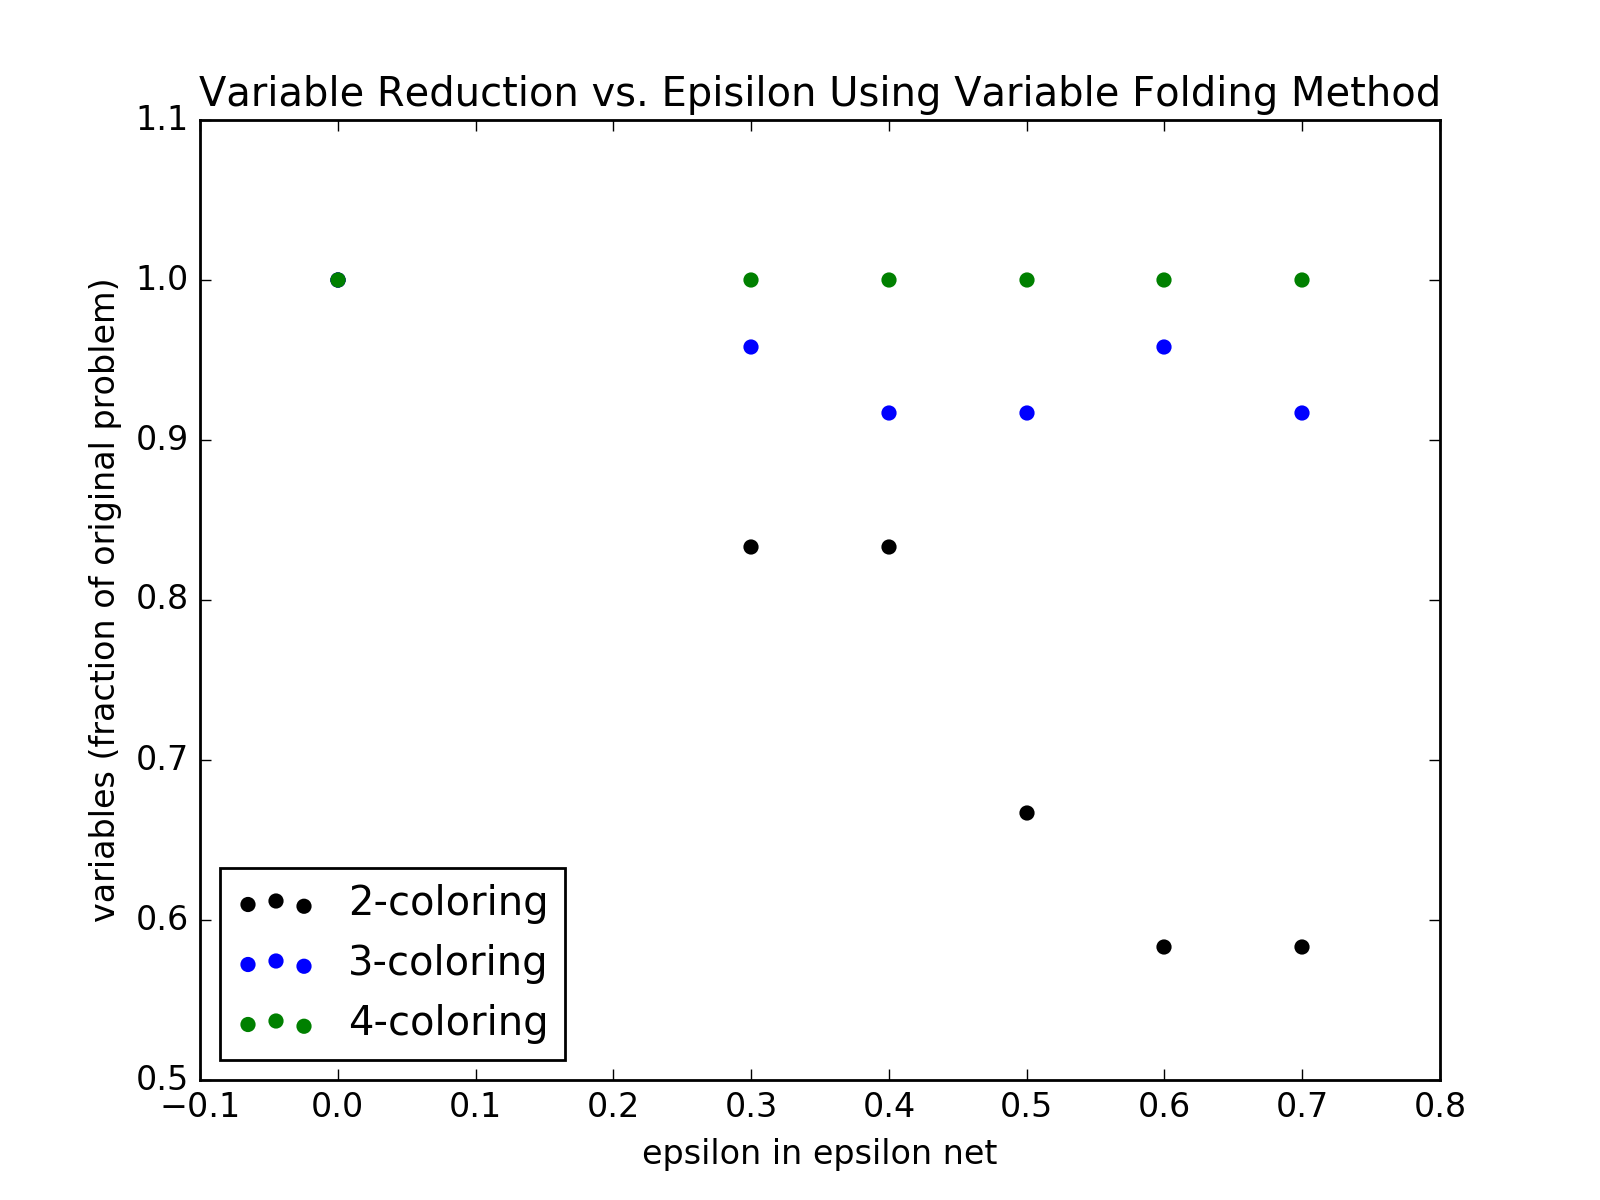
\includegraphics[width=\textwidth]{variables_epsilon_americas}
	\caption{Reduction in variables with variable folding method vs. epsilon and domain}
	\label{americas-reduction}
	\end{subfigure}
	~
	\begin{subfigure}[b]{0.45\textwidth}
	\centering
	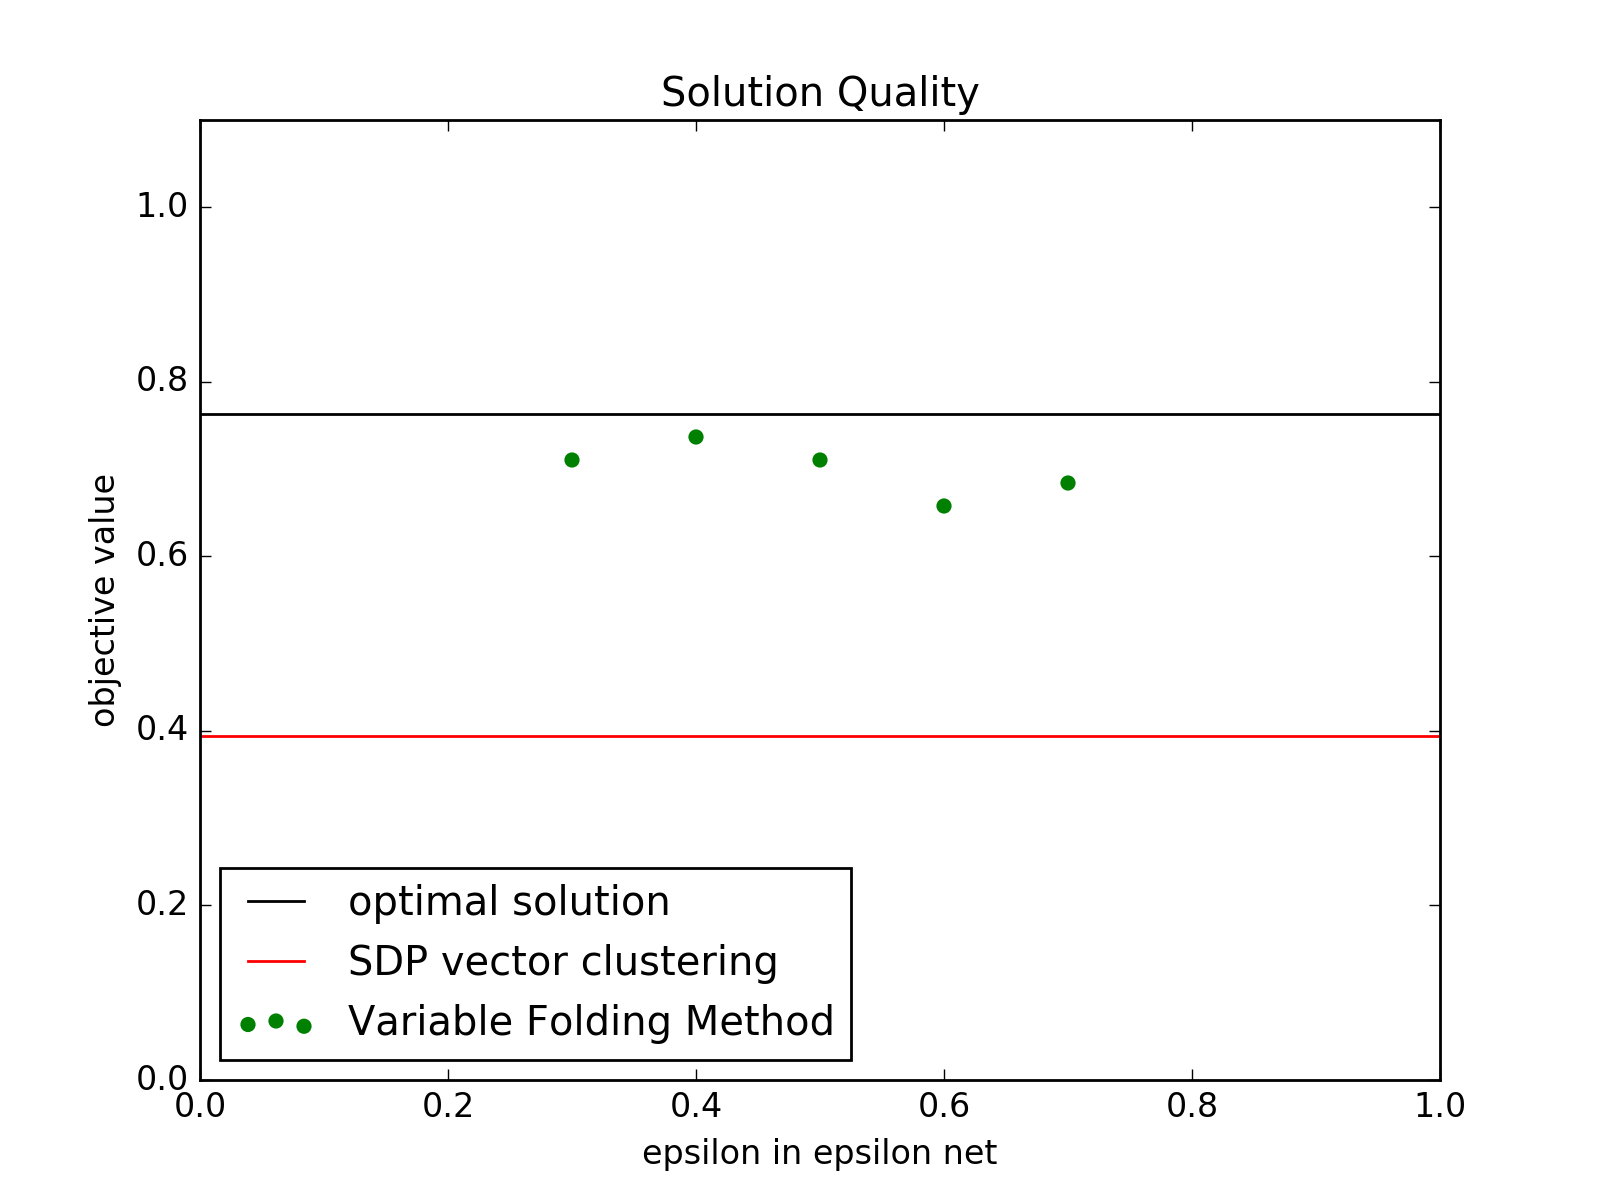
\includegraphics[width=\textwidth]{solution_epsilon_2coloring}
	\caption{Solution quality for 2-coloring the Americas}
	\label{2-coloring}
	\end{subfigure}

	\begin{subfigure}[b]{0.45\textwidth}
	\centering
	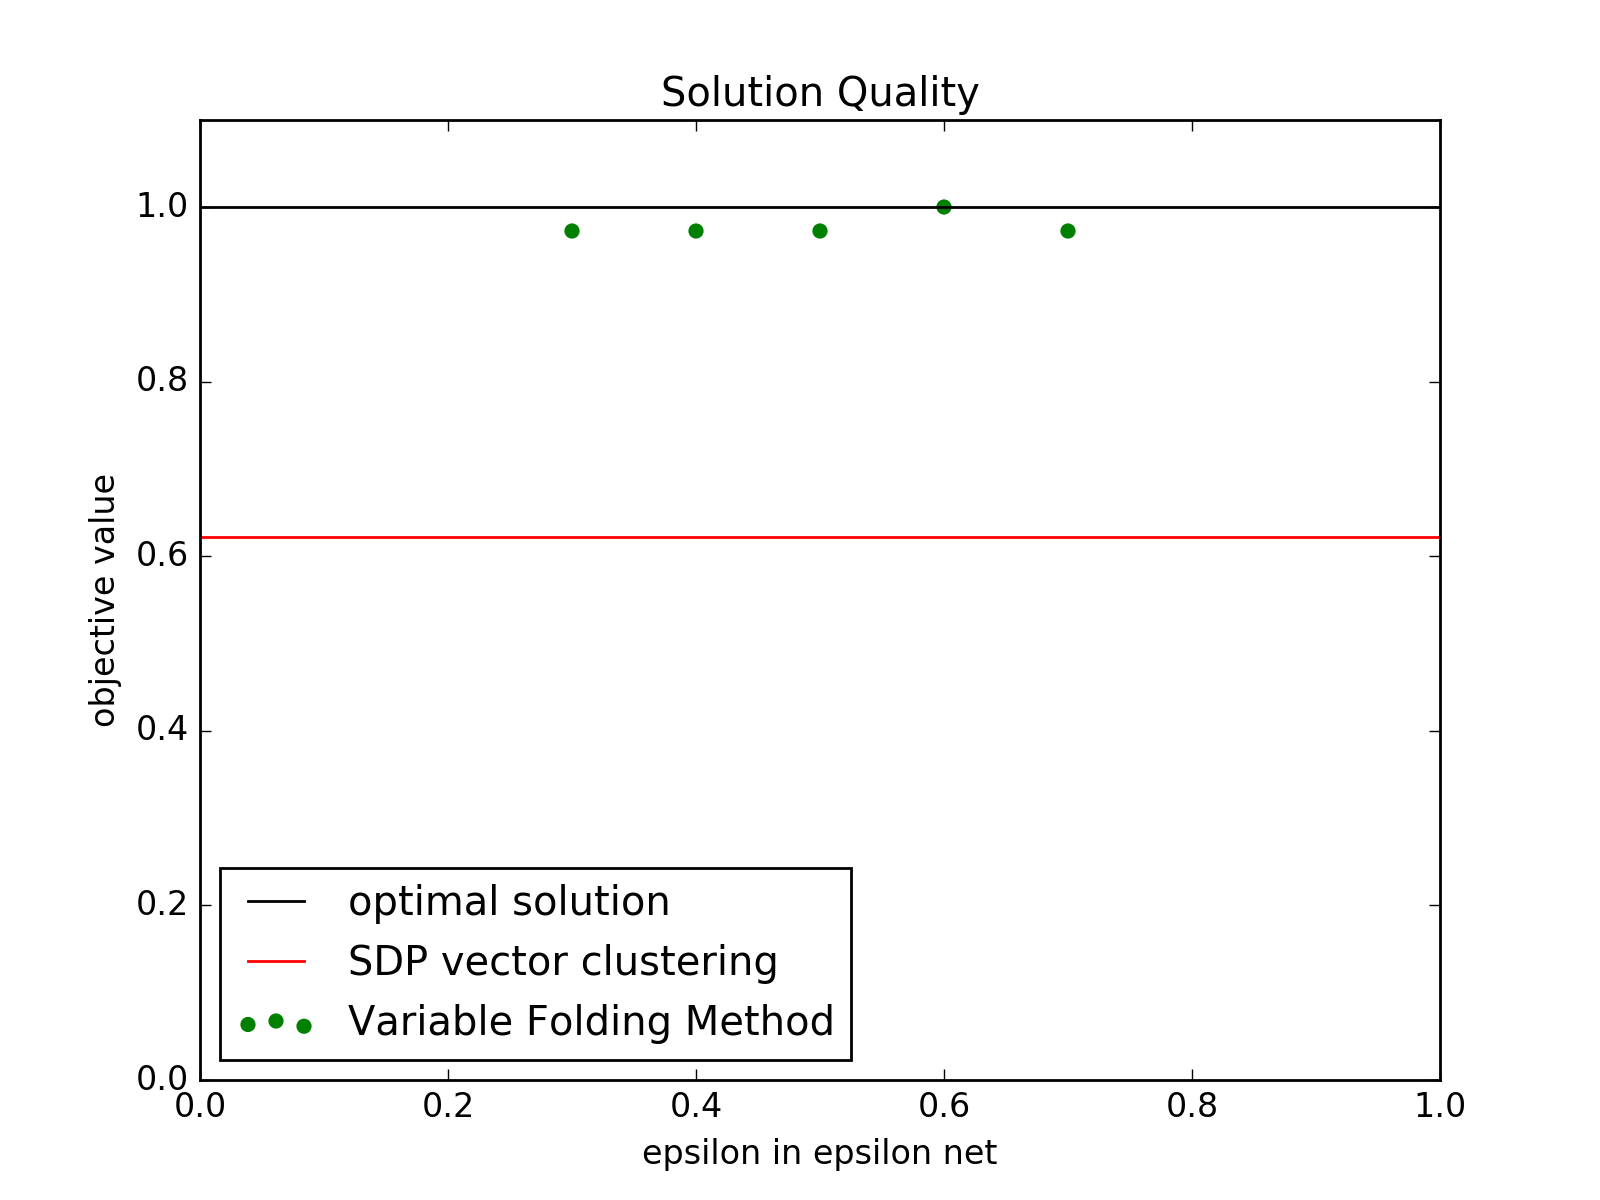
\includegraphics[width=\textwidth]{solution_epsilon_3coloring}
	\caption{Solution quality for 3-coloring the Americas}
	\label{3-coloring}
	\end{subfigure}
	~
	\begin{subfigure}[b]{0.45\textwidth}
	\centering
	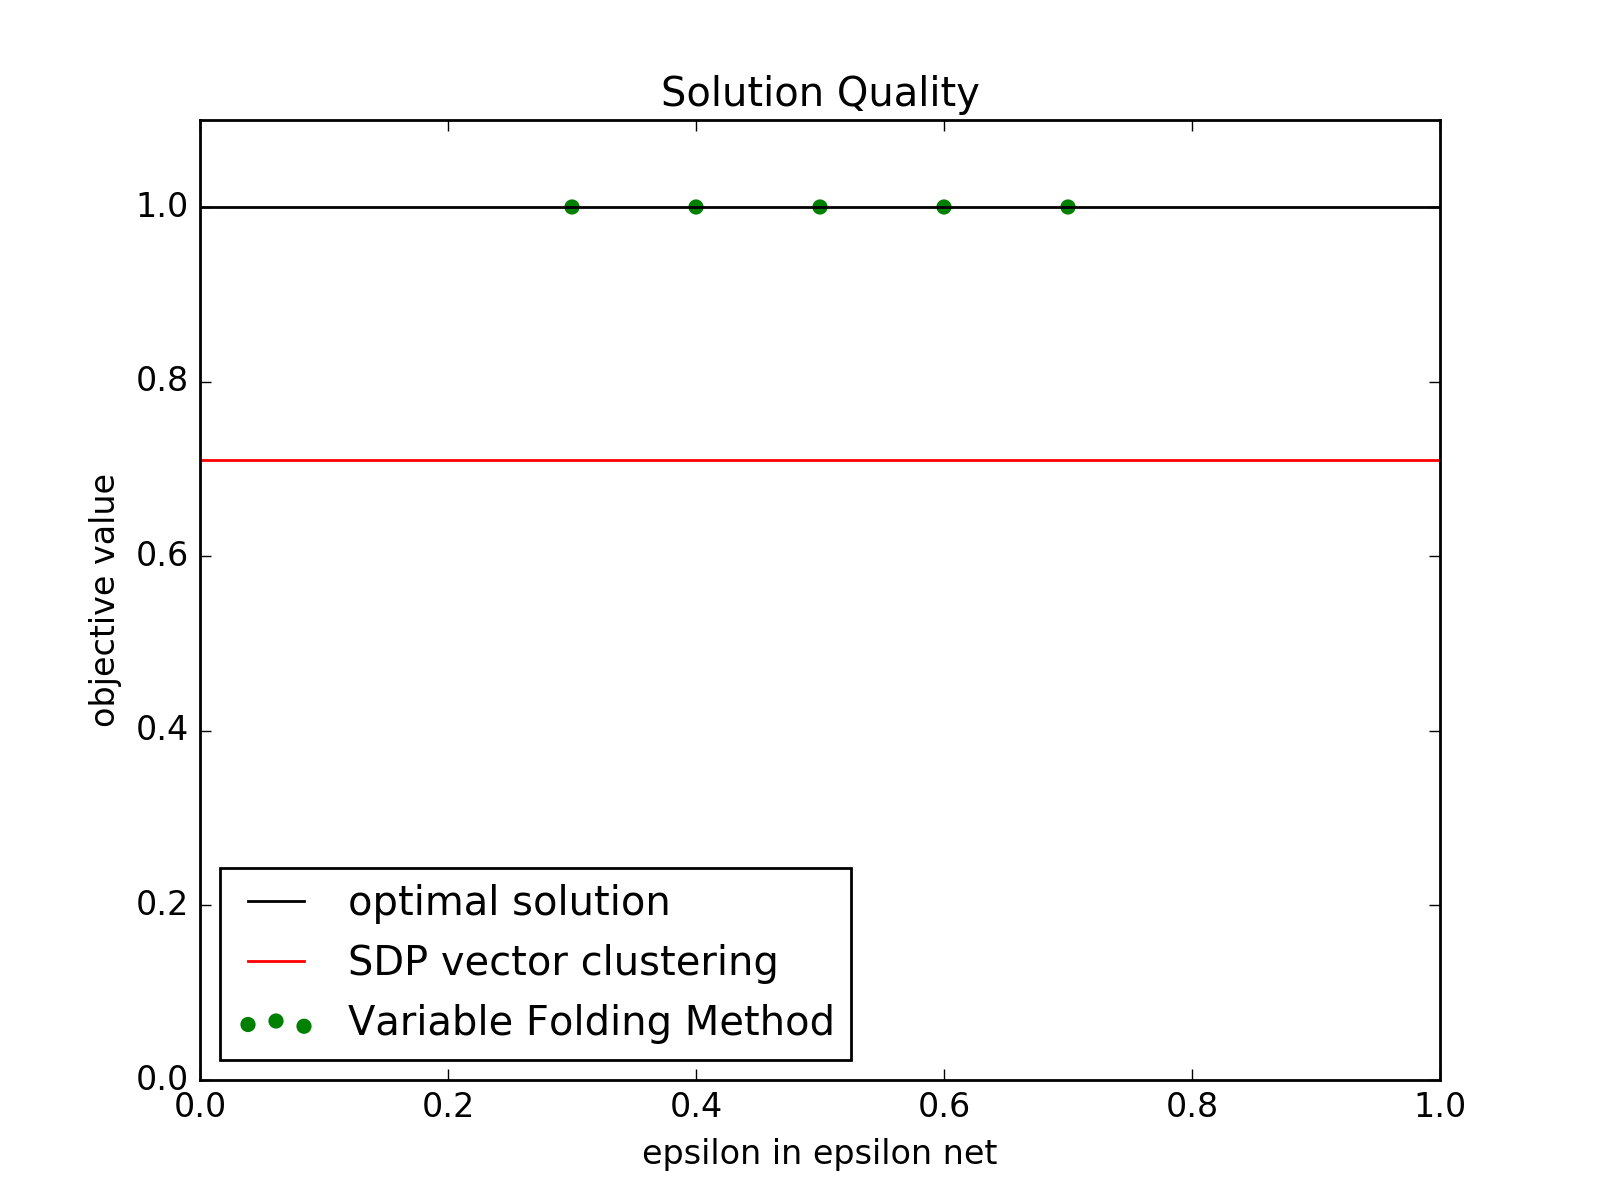
\includegraphics[width=\textwidth]{solution_epsilon_4coloring}
	\caption{Solution quality for 4-coloring the Americas}
	\label{4-coloring}
	\end{subfigure}
\caption{Evaluation of SDP Vector Clustering and the Variable Folding Method on the Americas Graph-Coloring Problem}
\label{americas}
\end{figure}

\begin{figure}[h!]
\centering
	\begin{subfigure}[b]{0.45\textwidth}
	\centering
	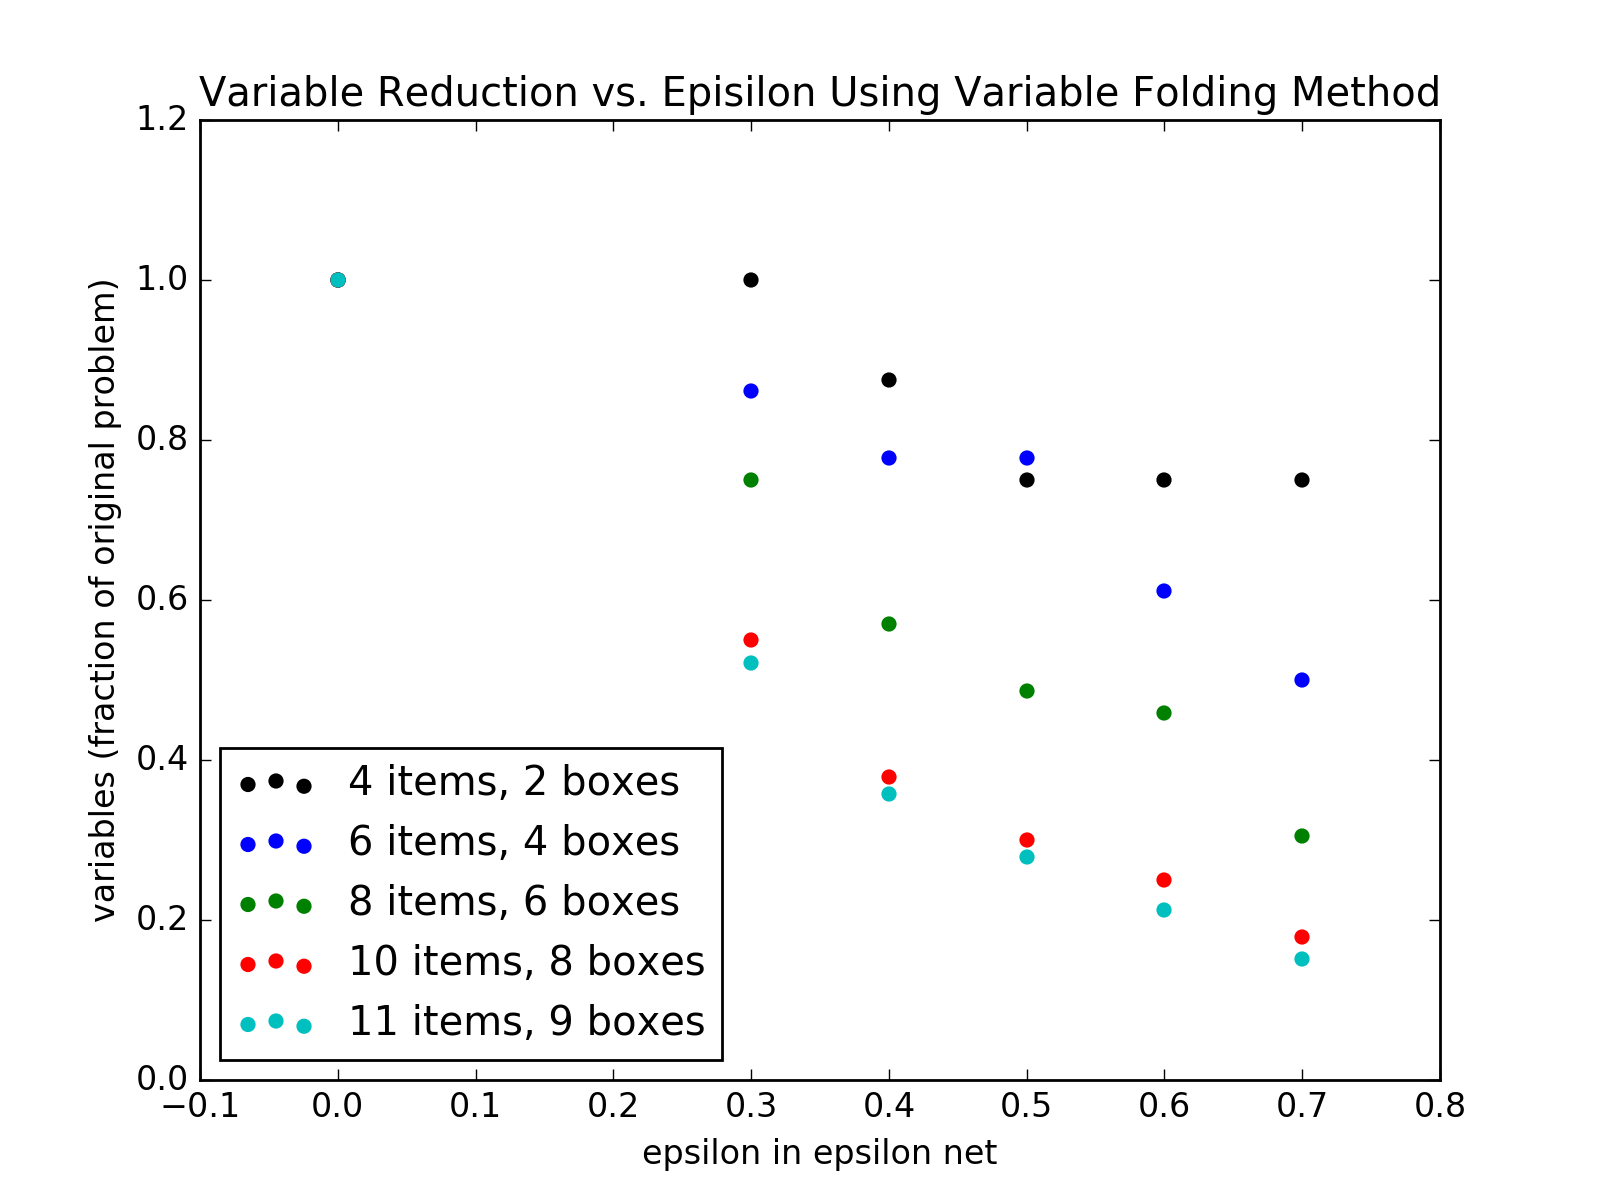
\includegraphics[width=\textwidth]{variables_epsilon_pigeon}
	\caption{Reduction in variables with variable folding method vs. epsilon and domain}
	\label{pigeon-reduction}
	\end{subfigure}
	~
	\begin{subfigure}[b]{0.45\textwidth}
	\centering
	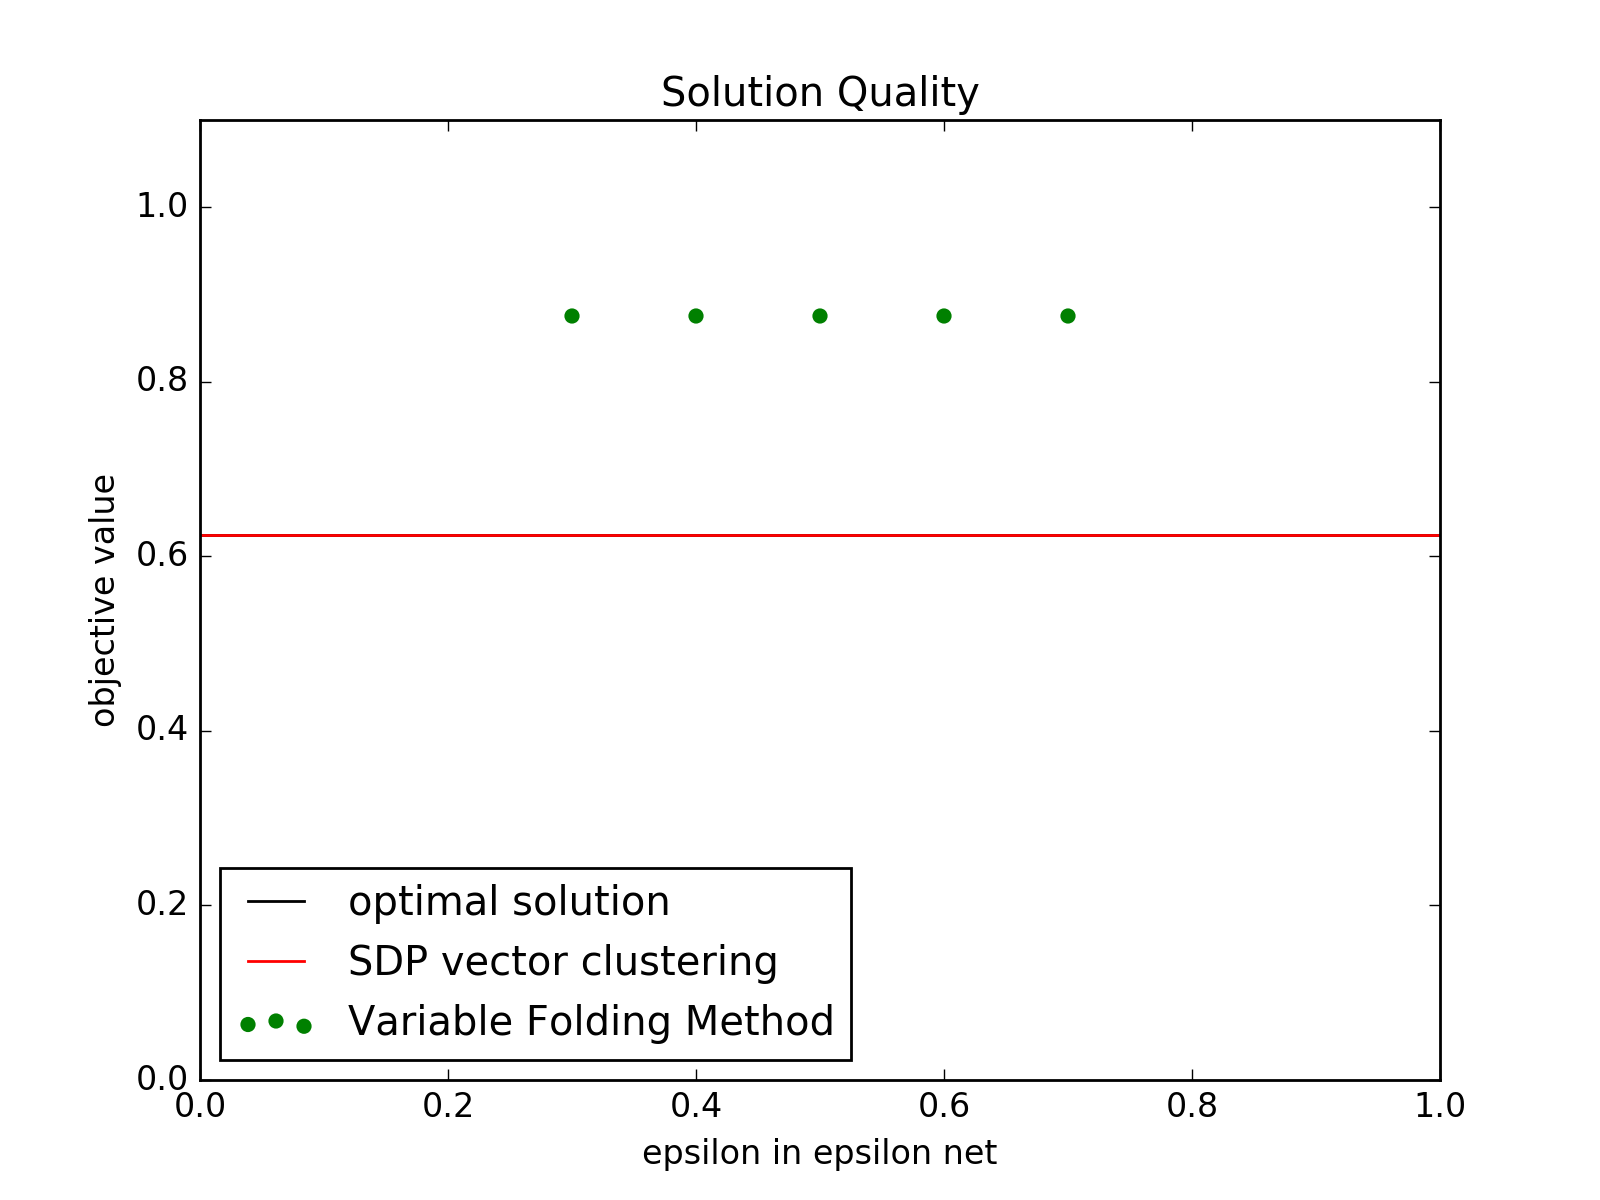
\includegraphics[width=\textwidth]{solution_epsilon_n4m2}
	\caption{Solution quality for 4 items in 2 boxes}
	\label{n4m2}
	\end{subfigure}

	\begin{subfigure}[b]{0.45\textwidth}
	\centering
	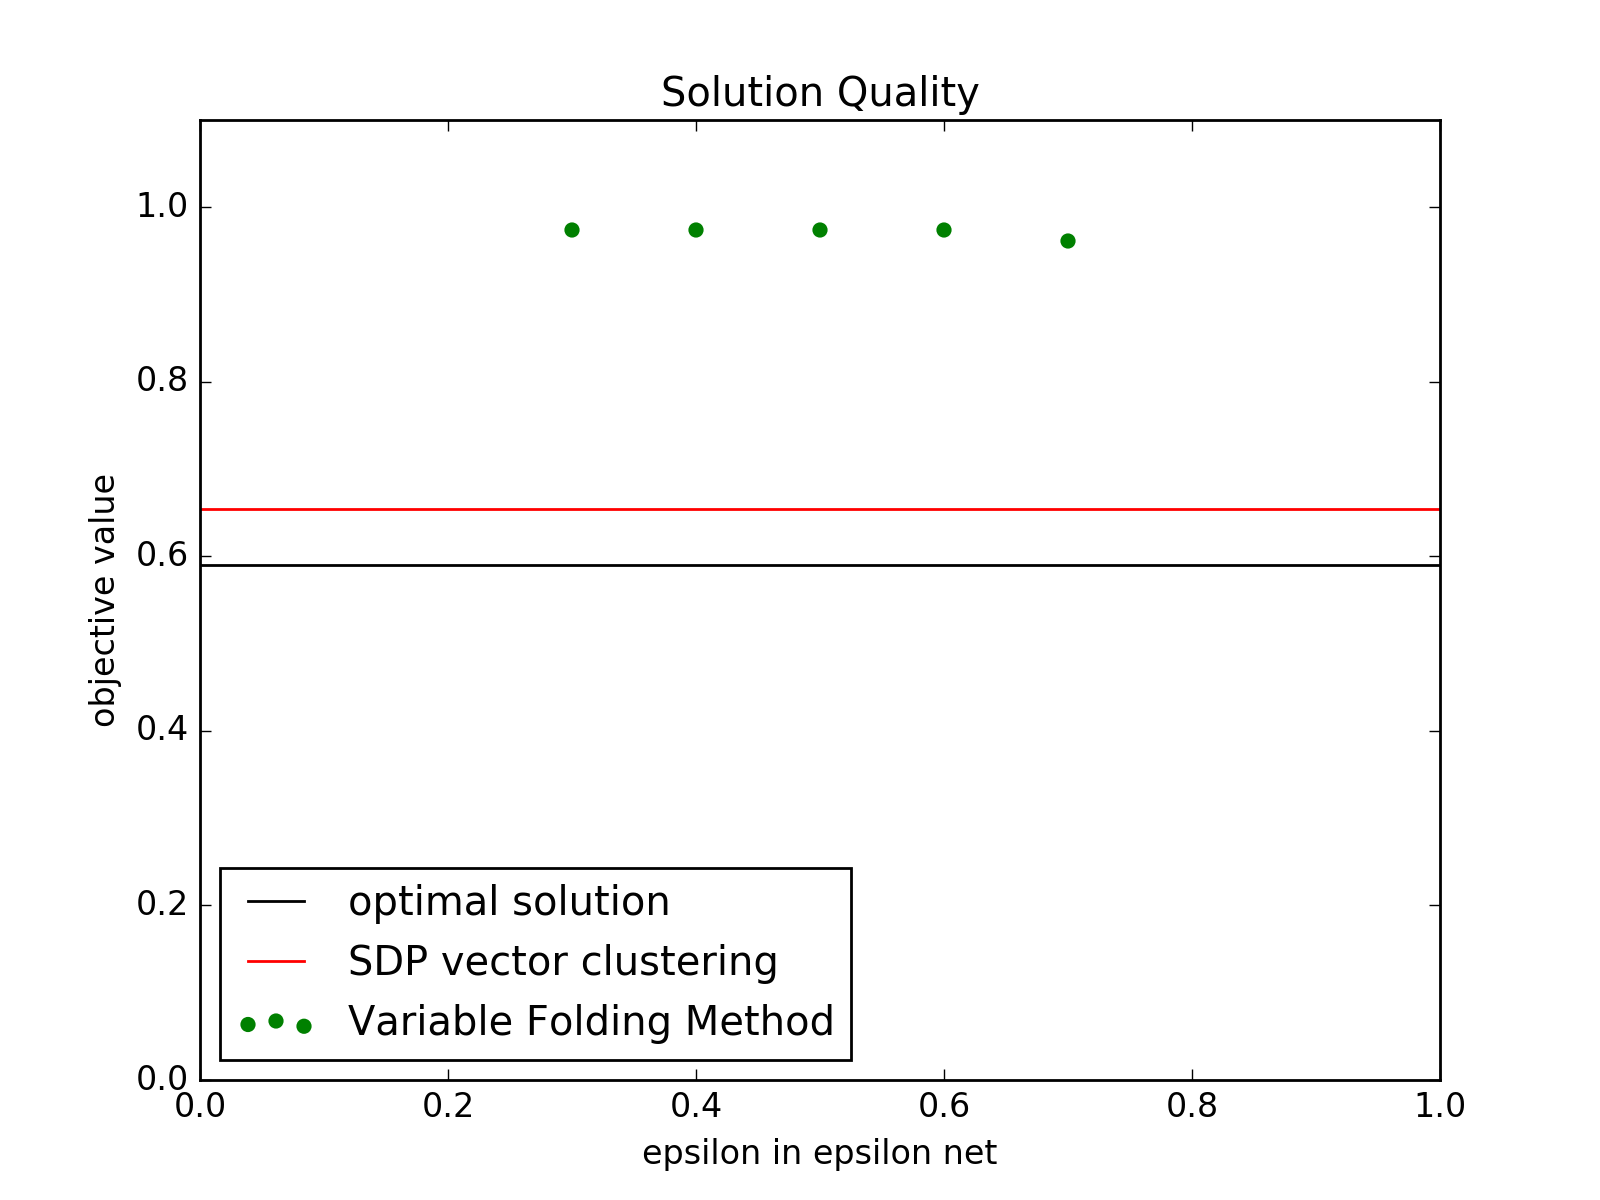
\includegraphics[width=\textwidth]{solution_epsilon_n6m4}
	\caption{Solution quality for 6 items in 4 boxes}
	\label{n6m4}
	\end{subfigure}
	~
	\begin{subfigure}[b]{0.45\textwidth}
	\centering
	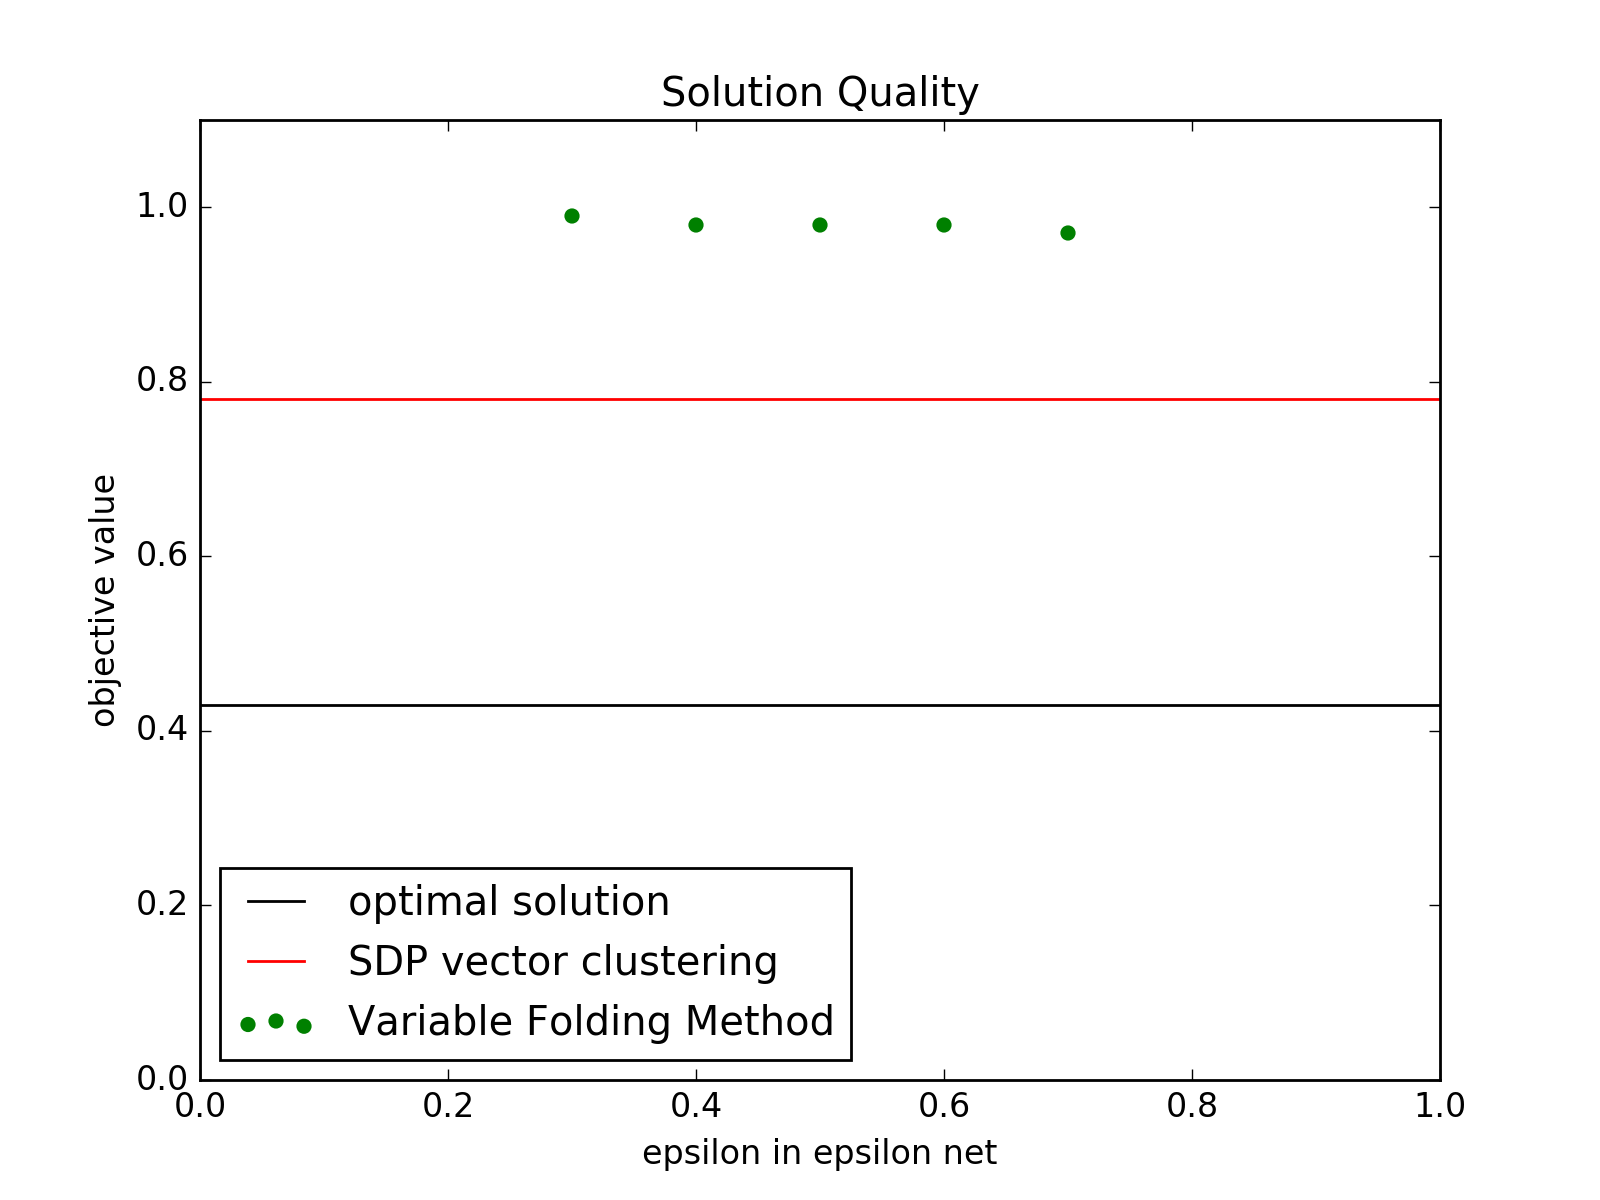
\includegraphics[width=\textwidth]{solution_epsilon_n8m6}
	\caption{Solution quality for 8 items in 6 boxes}
	\label{n8m6}
	\end{subfigure}

	\begin{subfigure}[b]{0.45\textwidth}
	\centering
	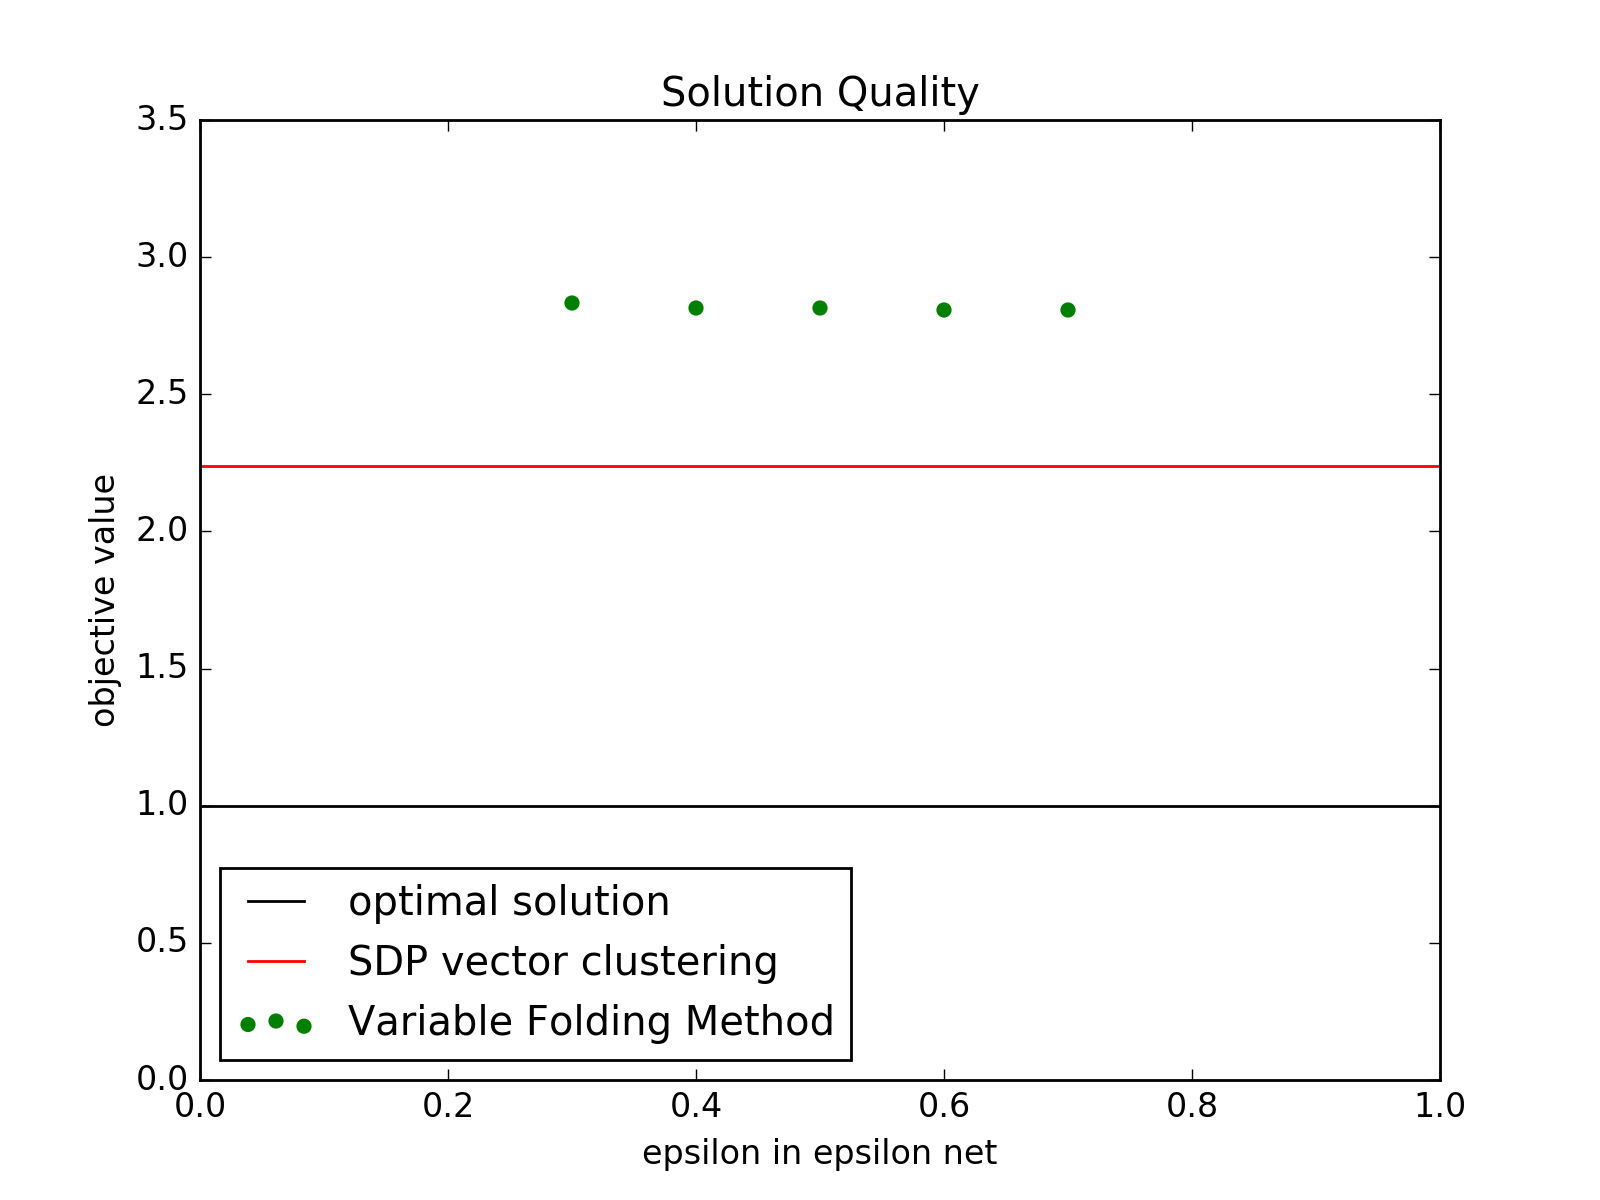
\includegraphics[width=\textwidth]{solution_epsilon_n10m8}
	\caption{Solution quality for 10 items in 8 boxes}
	\label{n10m8}
	\end{subfigure}
	~
	\begin{subfigure}[b]{0.45\textwidth}
	\centering
	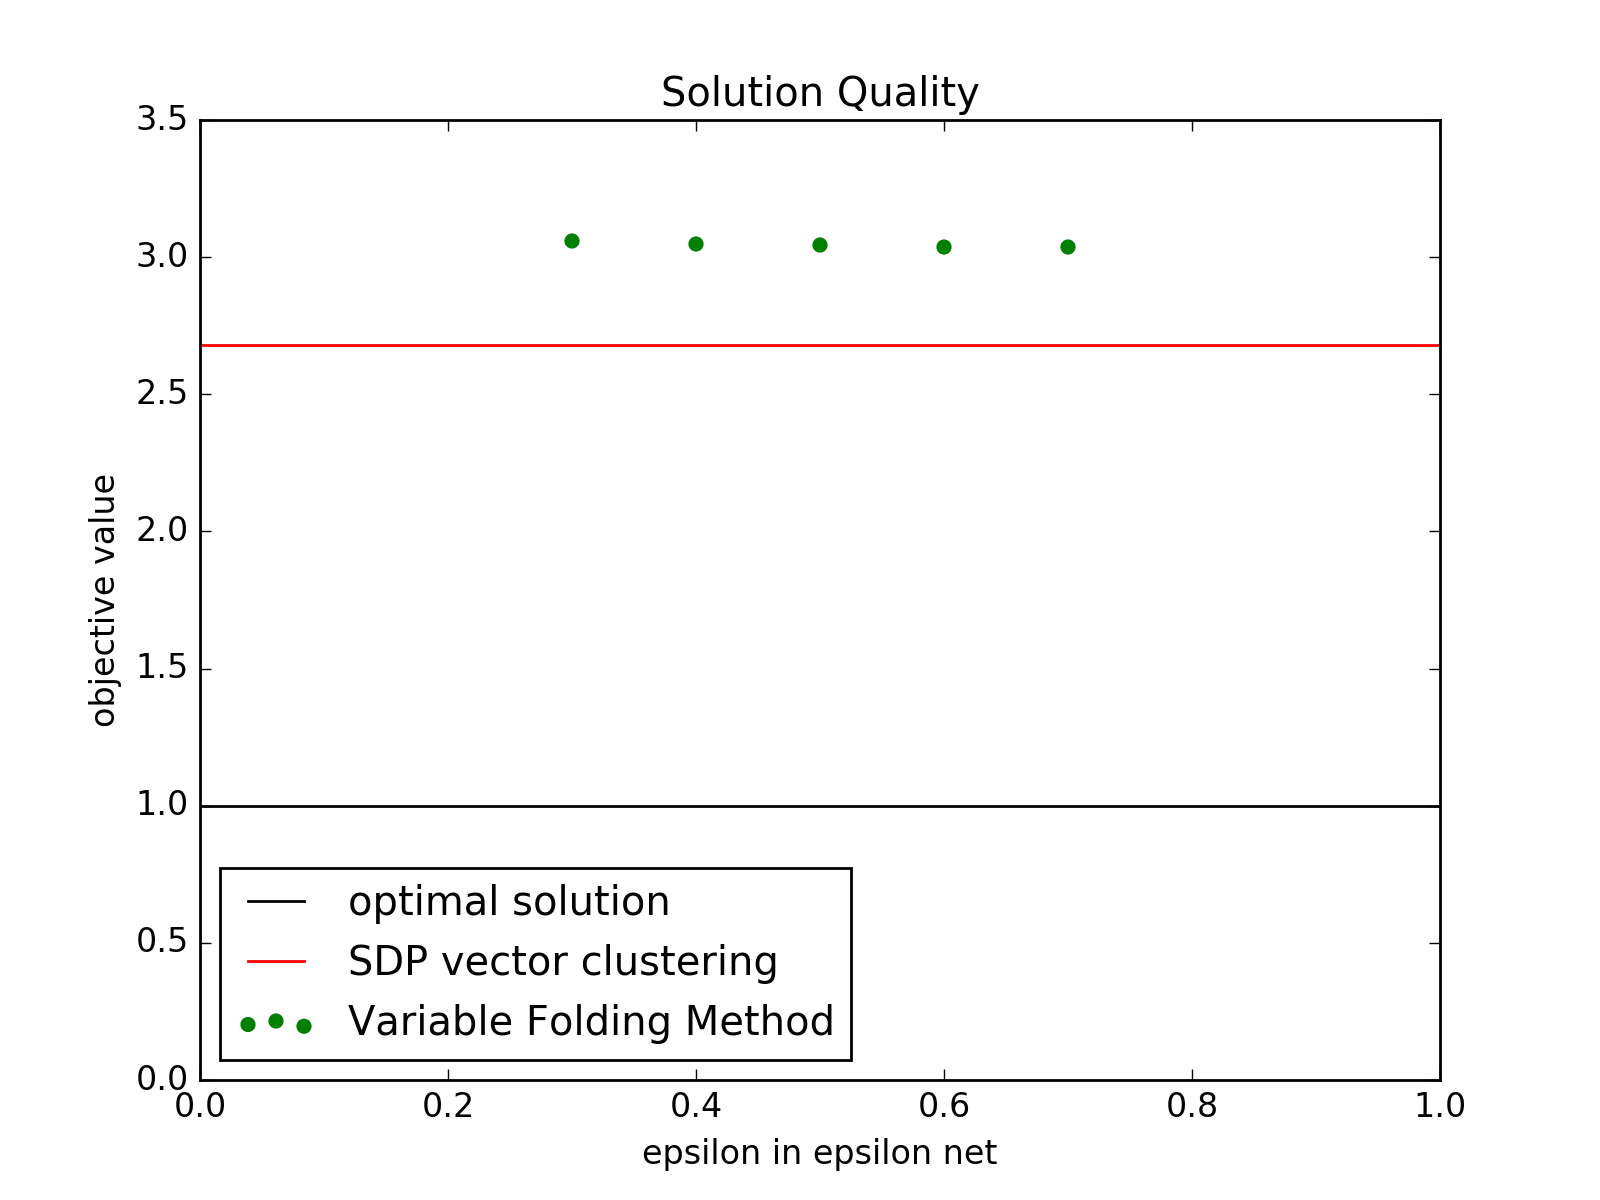
\includegraphics[width=\textwidth]{solution_epsilon_n11m9}
	\caption{Solution quality for 11 items in 9 boxes}
	\label{n11m9}
	\end{subfigure}
\caption{Evaluation of SDP Vector Clustering and the Variable Folding Method on the Pigeonhole Problem}
\label{pigeon}
\end{figure}

\section{Conclusion}

The two problems used to evaluate SDP vector clustering and the Variable Folding Method are favorable cases for SDP vector clustering because there are no constraints that reference specific values in the domain. In graph coloring, we simply want adjacent nodes to be different colors, and in the pigeonhole problem we want each box to contain no more than one item. If, for example, we wanted one node to be a particular color, or for one item to go in a specific box, then the assignment would affect the CSP objective. In the problems we tested, only the clustering process affects the CSP objective, not the assignment of values. If the assignment matters, then it is necessary to test all $|D|!$ possible assignments and the clustering method would be slower as a result.

%references
\renewcommand{\bibname}{References}
\bibliographystyle{apalike}
\bibliography{./227c_references}

\end{document}
